\chapter{Distributions of random variables}
\label{modeling}

\index{distribution!normal|(}

%_________________
\section{Normal distribution}\label{997}
\label{normalDist}

The probability density function of a standard normal random variable (one with mean $\E(X)=\mu=0$ and standard deviation $\SD(X)=\sigma=1$) is
\[
	f_Z(z) = \frac1{\sqrt{2\pi}} e^{-z^2/2},\quad -\infty<z<\infty.
\]
In general, if $X$ is normal with mean $\mu$ and variance $\sigma^2$ then
\[
	f_X(x) = \frac1{\sqrt{2\pi}\cdot\sigma} e^{-((x-\mu)/\sigma)^2/2},\quad -\infty<z<\infty.
\]
See Figure~\ref{simpleNormal}.

\begin{figure}
\centering
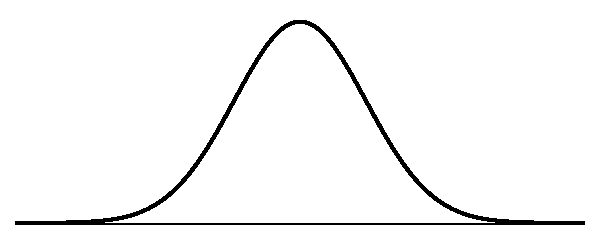
\includegraphics[width=0.7\textwidth]{ch_distributions/figures/simpleNormal/simpleNormal}
\caption{A normal curve.}
\label{simpleNormal}
\end{figure}

\begin{termBox}{\tBoxTitle{Normal distribution facts}
Variables appearing in nature are often nearly normal, but not exactly normal. This is due to the Central Limit Theorem stating that a sum of many (say $n$ many) independent and identically distributed random variables is approximately normally distributed (and that as the number $n\to\infty$, this approximation becomes as good as you like).\vspace{0.7mm}}
\end{termBox}

\begin{termBox}{\tBoxTitle{The Z-score}
The Z-score of an observation is the number of standard deviations it falls above or below the mean. We compute the Z-score for an observation $x$ that follows a distribution with mean $\mu$ and standard deviation $\sigma$ using
\begin{eqnarray*}
Z = \frac{x-\mu}{\sigma}
\end{eqnarray*}}
\end{termBox}

\subsection{Normal probability table}

Using Google Sheets' \sheets{normdist} and \sheets{norminv} is more practical than table look-up when a computer is handy.

Let us see how to reproduce the values in Table~\ref{zTableShort} using Google Sheets.

\sheets{=normdist(0.01,0,1,TRUE)}

gives the probability that $Z\le 0.01$ for a standard normal $Z$ (the TRUE referring to using the cumulative distribution function rather than the probability density function).

Here
\texttt{NORMDIST(x, mean, standard$\_$deviation, cumulative)}
has
\begin{itemize}
\item $x$ - The input to the normal function (whether probability density or cumulative distribution).
\item mean - The mean of the normal distribution function.
\item standard$\_$deviation - The standard deviation (sigma) of the normal distribution.
\item cumulative - Whether to use the cumulative distribution function rather than the probability density function.
\end{itemize}

\begin{table}
\centering
\begin{tabular}{c | rrrrr | rrrrr |}
  \cline{2-11}
&&&& \multicolumn{4}{c}{Second decimal place of $Z$} &&& \\
  \cline{2-11}
$Z$ & 0.00 & 0.01 & 0.02 & \highlightT{0.03} & \highlightO{0.04} & 0.05 & 0.06 & 0.07 & 0.08 & 0.09 \\
  \hline
  \hline
0.0 & \scriptsize{0.5000} & \scriptsize{0.5040} & \scriptsize{0.5080} & \scriptsize{0.5120} & \scriptsize{0.5160} & \scriptsize{0.5199} & \scriptsize{0.5239} & \scriptsize{0.5279} & \scriptsize{0.5319} & \scriptsize{0.5359} \\
  0.1 & \scriptsize{0.5398} & \scriptsize{0.5438} & \scriptsize{0.5478} & \scriptsize{0.5517} & \scriptsize{0.5557} & \scriptsize{0.5596} & \scriptsize{0.5636} & \scriptsize{0.5675} & \scriptsize{0.5714} & \scriptsize{0.5753} \\
  0.2 & \scriptsize{0.5793} & \scriptsize{0.5832} & \scriptsize{0.5871} & \scriptsize{0.5910} & \scriptsize{0.5948} & \scriptsize{0.5987} & \scriptsize{0.6026} & \scriptsize{0.6064} & \scriptsize{0.6103} & \scriptsize{0.6141} \\
%  May comment out 0.0-0.2 to make extra space. Then insert the following line:
%  $\vdots$ &   $\vdots$ &   $\vdots$ &   $\vdots$ &   $\vdots$ &   $\vdots$ &   $\vdots$ &   $\vdots$ &   $\vdots$ &   $\vdots$ &   $\vdots$ \\
  0.3 & \scriptsize{0.6179} & \scriptsize{0.6217} & \scriptsize{0.6255} & \scriptsize{0.6293} & \scriptsize{0.6331} & \scriptsize{0.6368} & \scriptsize{0.6406} & \scriptsize{0.6443} & \scriptsize{0.6480} & \scriptsize{0.6517} \\
\highlightT{0.4} & \scriptsize{0.6554} & \scriptsize{0.6591} & \scriptsize{0.6628} & \highlightT{\scriptsize{0.6664}} & \scriptsize{0.6700} & \scriptsize{0.6736} & \scriptsize{0.6772} & \scriptsize{0.6808} & \scriptsize{0.6844} & \scriptsize{0.6879} \\
  \hline
  0.5 & \scriptsize{0.6915} & \scriptsize{0.6950} & \scriptsize{0.6985} & \scriptsize{0.7019} & \scriptsize{0.7054} & \scriptsize{0.7088} & \scriptsize{0.7123} & \scriptsize{0.7157} & \scriptsize{0.7190} & \scriptsize{0.7224} \\
  0.6 & \scriptsize{0.7257} & \scriptsize{0.7291} & \scriptsize{0.7324} & \scriptsize{0.7357} & \scriptsize{0.7389} & \scriptsize{0.7422} & \scriptsize{0.7454} & \scriptsize{0.7486} & \scriptsize{0.7517} & \scriptsize{0.7549} \\
  0.7 & \scriptsize{0.7580} & \scriptsize{0.7611} & \scriptsize{0.7642} & \scriptsize{0.7673} & \scriptsize{0.7704} & \scriptsize{0.7734} & \scriptsize{0.7764} & \scriptsize{0.7794} & \scriptsize{0.7823} & \scriptsize{0.7852} \\
\highlightO{0.8} & \scriptsize{0.7881} & \scriptsize{0.7910} & \scriptsize{0.7939} & \scriptsize{0.7967} & \highlightO{\scriptsize{0.7995}} & \scriptsize{0.8023} & \scriptsize{0.8051} & \scriptsize{0.8078} & \scriptsize{0.8106} & \scriptsize{0.8133} \\
  0.9 & \scriptsize{0.8159} & \scriptsize{0.8186} & \scriptsize{0.8212} & \scriptsize{0.8238} & \scriptsize{0.8264} & \scriptsize{0.8289} & \scriptsize{0.8315} & \scriptsize{0.8340} & \scriptsize{0.8365} & \scriptsize{0.8389} \\
  \hline
  \hline
  1.0 & \scriptsize{0.8413} & \scriptsize{0.8438} & \scriptsize{0.8461} & \scriptsize{0.8485} & \scriptsize{0.8508} & \scriptsize{0.8531} & \scriptsize{0.8554} & \scriptsize{0.8577} & \scriptsize{0.8599} & \scriptsize{0.8621} \\
  1.1 & \scriptsize{0.8643} & \scriptsize{0.8665} & \scriptsize{0.8686} & \scriptsize{0.8708} & \scriptsize{0.8729} & \scriptsize{0.8749} & \scriptsize{0.8770} & \scriptsize{0.8790} & \scriptsize{0.8810} & \scriptsize{0.8830} \\
  $\vdots$ &   $\vdots$ &   $\vdots$ &   $\vdots$ &   $\vdots$ &   $\vdots$ &   $\vdots$ &   $\vdots$ &   $\vdots$ &   $\vdots$ &   $\vdots$ \\
   \hline
\end{tabular}
\caption{A section of the normal probability table. The percentile for a normal random variable with $Z=0.43$ has been \highlightT{highlighted}, and the percentile closest to 0.8000 has also been \highlightO{highlighted}.}
\label{zTableShort}
\end{table}

We can also find the Z-score associated with a percentile. For example, to identify Z for the $80^{th}$ percentile,
do
\noindent\texttt{=norminv(0.8,0,1)}
which yields 0.84.

\subsection{68-95-99.7 rule}

This useful rule of thumb for the probability of falling within 1, 2, and 3 standard deviations of the mean in the normal distribution is telling us values of
\[
\int_{-n}^n f_Z(z)\,dz
\]
where $f_Z(z)=\frac1{\sqrt{2\pi}} e^{-z^2/2}$ is the standard normal probability density function and $n\in\{1,2,3\}$. That is,
\begin{eqnarray*}
\int_{-1}^1 f_Z(z)\,dz &\approx& 68\%\\
\int_{-2}^2 f_Z(z)\, dz&\approx& 95\%\\
\int_{-3}^3 f_Z(z)\, dz&\approx& 99.7\%
\end{eqnarray*}
As there is no elementary antiderivative for $e^{-z^2/2}$, these integrals are calculated by \emph{numerical integration} that you may recall from a calculus course.

%Zain:
We may consider Taylor series as one way of approximating. Recalling that $e^x=\sum_{n=0}^\infty x^n/n!$, it follows that
\[
	e^{-x^2/2} = \sum_{n=0}^\infty \frac{(-1)^n x^{2n}}{2^n n!}.
\]
Integrating this term by term, we have
\begin{eqnarray*}
	\int e^{-x^2/2}\,dx &=& \sum_{n=0}^\infty \frac{(-1)^n x^{2n+1}}{(2n+1)2^n n!} + \text{constant} \\
	&\approx& x -\frac{x^3}{6} +C.
\end{eqnarray*}
For the standard normal cdf $\Phi$ we want $\Phi(0)=1/2$, which means
\[
	\Phi(x)\approx \frac1{\sqrt{2\pi}} \left(x-\frac{x^3}6\right)+\frac12
\]
for $x\approx 0$.
To see how good this approximation is, let us compute
\[
	68\% \approx \Phi(1)-\Phi(-1)\approx \frac1{\sqrt{2\pi}}\left(2-\frac26\right)=\frac1{\sqrt{2\pi}}\frac53 = .6649
\]
which is not bad.

Let us also try using Simpson' Rule: with $f=f_Z$, $\Delta x = 1$, and $(x_0,x_1,x_2)=(-1,0,1)$, we have
\begin{eqnarray*}
	\int_{-1}^1 f_Z(z)\,dz &\approx& \frac{\Delta x}3 \left(f(x_0)+4f(x_1)+f(x_2)\right)\\
	&=&\frac13\frac1{\sqrt{2\pi}} (e^{-(-1)^2/2} + 4e^{-0^2/2} + e^{-(1)^2/2})\\
	&=& \frac1{3\sqrt{2\pi}} (2e^{-1/2}+4)\\
	&=& \frac{\sqrt{2}}{3\sqrt{\pi e}}(1+2\sqrt{e})\\
	&\approx& .6932\dots
\end{eqnarray*}
and with $(x_0,x_1,x_2,x_3,x_4)=(-2,-1,0,1,2)$, we have
\begin{eqnarray*}
	\int_{-2}^2 f_Z(z)\,dz &\approx& \frac{\Delta x}3 \left(f(x_0)+4f(x_1)+2f(x_2)+4f(x_3)+f(x_4)\right)\\
	&=& \frac1{3\sqrt{2\pi}} \left(e^{-4/2} + 4 e^{-1/2} + 2 e^{-0/2} + 4 e^{-1/2} + e^{-4/2}\right)\\
	&=&\frac1{3\sqrt{2\pi}}\left(2e^{-2} + 8e^{-1/2} + 2\right)\\
	&\approx& .9472\dots
\end{eqnarray*}

\begin{figure}%[hht]
\centering
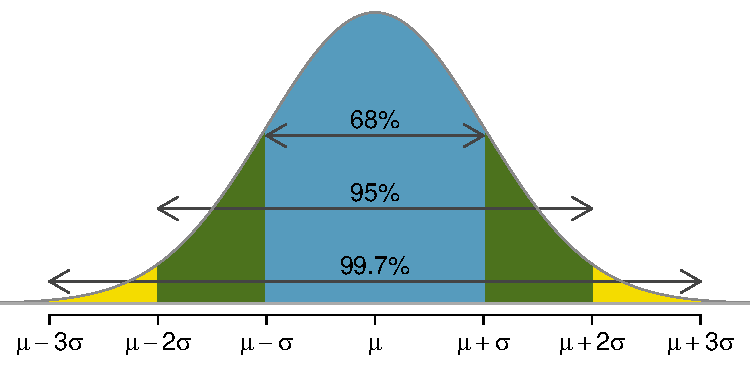
\includegraphics[height=1.9in]{ch_distributions/figures/6895997/6895997}
\caption{Probabilities for falling within 1, 2, and 3 standard deviations of the mean in a normal distribution.}
\label{6895997}
\end{figure}


%_________________
\subsection{Normal probability plots}
\label{assessingNormal}

%supplement start

To make a normal probability plots, proceed as follows.
\begin{itemize}
\item Using the mean and (sample) standard deviation, standardize the data set.
\item Construct the \term{empirical cdf} which is just the cdf of the uniform distribution on the data set we are working with.
\item In Google Sheets, highlight two columns with the values of the empirical and normal cdfs (using \texttt{normdist} function with cdf set to 1 or True) at the values in our data set.
\item Display a scatter plot of these two columns. That is our normal probability plot.
\end{itemize}
%supplement end
\index{normal probability plot|)}
\index{distribution!normal|)}


\section{Bernoulli distribution}
\label{bernoulli}

\index{distribution!Bernoulli|(}

\begin{termBox}{\tBoxTitle{Bernoulli random variable, descriptive}
A Bernoulli random variable has exactly two possible outcomes. We typically label one of these outcomes a ``success'' and the other outcome a ``failure''. We may also denote a success by \resp{1} and a failure by \resp{0}.}
\end{termBox}

In a way, the Bernoulli distribution is too simple to be of much use by itself. On the other hand, sums of independent Bernoulli's give us the binomial distribution $\sum_i X_i$ which approximates the normal distribution and can be used for estimating proportions such as voter support and disease prevalence. The Bernoulli distribution is just complicated enough that its sample averages $\sum_{i=1}^n X_i/n$ are interesting.

Bernoulli random variables are often denoted as \resp{1} for a success and \resp{0} for a failure. In addition to being convenient in entering data, it is also mathematically handy. Suppose we observe ten trials:
\begin{center}
\resp{0} \resp{1} \resp{1} \resp{1} \resp{1} \resp{0} \resp{1} \resp{1} \resp{0} \resp{0}
\end{center}
Then the \term{sample proportion}, $\hat{p}$, is the sample mean of these observations:
\begin{eqnarray*}
\hat{p} = \frac{\text{\# of successes}}{\text{\# of trials}} = \frac{0+1+1+1+1+0+1+1+0+0}{10} = 0.6
\end{eqnarray*}%

This mathematical inquiry of Bernoulli random variables can be extended even further. Because \resp{0} and \resp{1} are numerical outcomes, we can define the {mean} and {standard deviation} of a Bernoulli random variable. If ${p}$ is the true probability of a success, then the mean of a Bernoulli random variable $X$ is given by
\begin{align*}
\mu = \E[X] &= \P(X=0)\times0 + \P(X=1)\times1 \\
	&= (1-p)\times0 + p\times 1 = 0+p = p
\end{align*}
Similarly, the variance of $X$ can be computed:
\begin{align*}
\Var(X)=\sigma^2 &= {\P(X=0)(0-p)^2 + \P(X=1)(1-p)^2} \\
	&= {(1-p)p^2 + p(1-p)^2} = {p(1-p)}
\end{align*}
The standard deviation is $\SD(X)=\sigma=\sqrt{p(1-p)}$.

\begin{termBox}{\tBoxTitle{Bernoulli random variable, mathematical}
If $X$ is a random variable that takes value 1 with probability of success $p$ and 0 with probability $1-p$, then $X$ is a Bernoulli random variable with mean and standard deviation
\begin{align*}
\mu &= p
	&\sigma&= \sqrt{p(1-p)}
\end{align*}}
\end{termBox}

In general, it is useful to think about a Bernoulli random variable as a random process with only two outcomes: a success or failure. Then we build our mathematical framework using the numerical labels \resp{1} and \resp{0} for successes and failures, respectively.

\index{distribution!Bernoulli|)}

\section{Geometric distribution}\label{geomDist}


\index{distribution!geometric|(}

We now derive the formulas for the mean (expected) number of trials needed to find the first success and the standard deviation or variance of this distribution.

\begin{termBox}{\tBoxTitle{Geometric Distribution\index{distribution!geometric|textbf}}
If the probability of a success in one trial is $p$ and the probability of a failure is $1-p$, then the probability of finding the first success in the $n^{th}$ trial is given by\vspace{-1.5mm}
\begin{eqnarray}
(1-p)^{n-1}p
\end{eqnarray}
The mean (i.e. expected value), variance, and standard deviation of this wait time are given by\vspace{-2.5mm}
\begin{align}
\mu &= \frac{1}{p}
	&\sigma^2&=\frac{1-p}{p^2}
	&\sigma &= \sqrt{\frac{1-p}{p^2}}
\label{geomFormulas}
\end{align}}
\end{termBox}

%\begin{exercise}
%Using the results from Example~\ref{onlyShocking55PercOfTheTimeExample}, $\mu = 2.22$ and $\sigma = 1.65$, would it be appropriate to use the normal model to find what proportion of experiments would end in 3 or fewer trials?\footnote{No. The geometric distribution is always right skewed and can never be well-approximated by the normal model.}
%\end{exercise}

\index{distribution!geometric|)}

%SUPPLEMENT START
Note that the variance $\sigma^2$ of a random variable $X$ has the relatively simple formula $\sigma^2=\E(X^2)-(\E(X))^2$, as we verify as follows:
\begin{eqnarray*}
\sigma^2 &=& \E((X-\E(X))^2) = \E(X^2 - 2X\E(X) + (\E(X))^2)\\
&=& \E(X^2) - 2(\E(X))^2 + (\E(X))^2 = \E(X^2)-(\E(X))^2.
\end{eqnarray*}

We can verify the important property $\P(-\infty<X<\infty)=1$ of probability distributions in the geometric case as follows.
First recall the geometric series
\[
	\sum_{n=0}^\infty x^n = \frac{1}{1-x},\quad |x|<1
\]
Then
\begin{eqnarray*}
\P(1\le X<\infty) = \sum_{k=1}^\infty \P(X=k) &=& \sum_{k=1}^\infty (1-p)^{k-1}p\\
 &=& \sum_{t=0}^\infty (1-p)^t p = p\cdot \frac{1}{1-(1-p)} = 1.
\end{eqnarray*}
\begin{thm}
The mean of a geometric random variable $X$ is $1/p$.
\end{thm}
\begin{proof}
First let us recall (or learn) another series from Calculus:
\[
	\alpha := \sum_{n=0}^\infty n x^n = \sum_{n=0}^\infty (n+1) x^{n+1} = \sum_{n=0}^\infty n x^{n+1} + \sum_{n=0}^\infty x^{n+1} = \alpha\cdot x + \left(\frac1{1-x}-1\right),
\]
so we can solve for $\alpha$ and get
\[
\alpha = \frac{\frac1{1-x}-1}{1-x} = \frac{1-(1-x)}{(1-x)^2} = \frac{x}{(1-x)^2}.
\]
Therefore,
\begin{eqnarray*}
\E(X)=\sum_{k=1}^\infty k \P(X=k)&=&\sum_{k=1}^\infty k (1-p)^{k-1}p\\
&=&\frac{p}{1-p}\sum_{k=0}^\infty k(1-p)^k = \frac{p}{1-p} \cdot \frac{1-p}{p^2} = \frac1{p}.\qedhere
\end{eqnarray*}
\end{proof}
\begin{thm}\label{varGeom}
The variance of a geometric random variable $X$ is $\frac{1-p}{p^2}$.
\end{thm}
\begin{proof}
Let
\[
	\beta := \sum_{n=0}^\infty n^2 x^n = \sum_{n=0}^\infty (n+1)^2 x^{n+1} = \sum_{n=0}^\infty (n^2+2n+1) x^{n+1} = x\left(\beta+2\alpha+\frac{1}{1-x}\right)
\]
Solving this for $\beta$ and using $\sigma^2=\E(X^2)-(\E(X))^2$ we get our formula for $\sigma$; see Exercise \ref{verifying_the_variance}.
\end{proof}
%SUPPLEMENT END

\section{Binomial distribution}
\label{binomialModel}

\index{distribution!binomial|(}


%\textC{\newpage}


%\subsection{The binomial distribution}

The \termsub{binomial distribution}{distribution!binomial} describes the probability of having exactly $k$ successes in $n$ independent Bernoulli trials with probability of a success $p$.

%Here we shall derive the formulas for $n\choose k$, and mean and variance of the binomial distribution.
%We shall also discuss the $np\ge 10$, $n(1-p)\ge 10$ rule.
The quantity
\begin{eqnarray*}
{n\choose k} = \frac{n!}{k!(n-k)!}
\end{eqnarray*}
is read \term{n choose k}.\footnote{Other notation for $n$ choose $k$ includes $_nC_k$, $C_n^k$, and $C(n,k)$.} The exclamation point notation (e.g. $k!$) denotes a \term{factorial}\label{factorialDefinitionInTheBinomialSection} expression (Table \ref{factorialTable}).

\begin{table}
\centering
\begin{tabular}{| r | r |}
\hline
$n$ & $n!$\\
\hline
0&1\\
1&1\\
2&2\\
3&6\\
4&24\\
5&120\\
6&720\\
7&5040\\
8&40320\\
\hline
\end{tabular}
\caption{How many of these do you remember? An urban legend says that undergraduates know that $3!=6$, graduate students that $4!=24$, postdocs that $5!=120$,
and professors that $6!=720$.}\label{factorialTable}
\end{table}

\begin{thm}
$\binom{n}{k}$ equals the number of subsets $F$ of an $n$-element set $[n]:=\{1,\dots,n\}$ such that $F$ has $k$ elements.
\end{thm}
\begin{proof}[Proof idea]
The number of sequences $(a_1,\dots,a_k)$ where all the $a_i$ are distinct and coming from $[n]$, is $n!/(n-k)!$. Indeed, we have $n$ choices for $a_1$, then $n-1$ choices for $a_2$ given a choice of $a_1$, and so on. A set $F$ is represented by $k!$ such sequences.
\end{proof}
\begin{example}{Understanding binomial coefficients.}
We have $\binom42=6$ because the 2-element subsets of [4] are the following six:
\[
	\{1,2\}, \{1,3\}, \{1,4\}, \{2,3\}, \{2,4\}, \{3,4\}.
\]
We have $\binom41=4$ because the 1-element subsets of [4] are the following four:
\[
	\{1\}, \{2\}, \{3\}, \{4\}.
\]
We have $\binom40=1$ because there is exactly one 0-element subset of [4]:
\[
	\emptyset.
\]
We have $\binom43=4$ because there are exactly four 3-element subsets of [4]:
\[
	\{1,2,3\}, \{1,2,4\}, \{1,3,4\}, \{2,3,4\}.
\]
Finally, we have $\binom44=1$ as there is only one 4-element subset of [4]:
\[
	\{1,2,3,4\}.
\]
Finally, $\sum_{i=0}^4\binom4i=16=2^4$ collects all these 16 subsets.
\end{example}

\begin{termBox}{\tBoxTitle{Binomial distribution} Suppose the probability of a single trial being a success is $p$. Then the probability of observing exactly $k$ successes in $n$ independent trials is given by\vspace{-1mm}
\begin{eqnarray}
{n\choose k}p^k(1-p)^{n-k} = \frac{n!}{k!(n-k)!}p^k(1-p)^{n-k}
\label{binomialFormula}
\end{eqnarray}
Additionally, the mean, variance, and standard deviation of the number of observed successes are\vspace{-2mm}
\begin{align}
\mu &= np
	&\sigma^2 &= np(1-p)
	&\sigma &= \sqrt{np(1-p)}
\label{binomialStats}
\end{align}}
\end{termBox}



%\subsection{Normal approximation to the binomial distribution}
\label{normalApproxBinomialDistSubsection}

\index{distribution!binomial!normal approximation|(}

The binomial formula is cumbersome when the sample size ($n$) is large, particularly when we consider a range of observations. In some cases we may use the normal distribution as an easier and faster way to estimate binomial probabilities.

%\begin{figure}%[h]
%\centering
%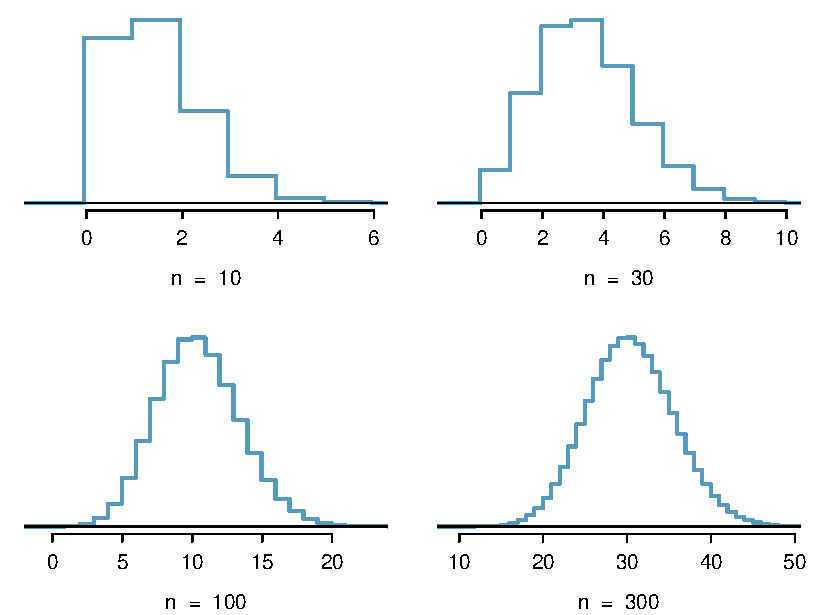
\includegraphics[width=0.92\textwidth]{ch_distributions/figures/fourBinomialModelsShowingApproxToNormal/fourBinomialModelsShowingApproxToNormal}
%\caption{Hollow histograms of samples from the binomial model when $p=0.10$. The sample sizes for the four plots are $n=10$, 30, 100, and 300, respectively.}
%\label{fourBinomialModelsShowingApproxToNormal}
%\end{figure}

\begin{termBox}{\tBoxTitle{Normal approximation of the binomial distribution}
The binomial distribution with probability of success $p$ is nearly normal when the sample size $n$ is sufficiently large that $np$ and $n(1-p)$ are both at least 10. The approximate normal distribution has parameters corresponding to the mean and standard deviation of the binomial distribution:\vspace{-1.5mm}
\begin{align*}
\mu &= np
&&\sigma= \sqrt{np(1-p)}
\end{align*}}
\end{termBox}


\paragraph{The 10\% condition.}
When drawing a sample from a larger population, the \term{10\% condition} helps our samples to be independent. If our sample has more than 10\% of the individuals, then knowing that 5\% has a certain property may mean that the other 5\% cannot have this property. See also Section \ref{tenpercent}.


%\subsection{The normal approximation breaks down on small intervals}

\begin{caution}
{The normal approximation may fail on small intervals}
{The normal approximation to the binomial distribution tends to perform poorly when estimating the probability of a small range of counts, even when the conditions are met.}
\end{caution}

%Suppose we wanted to compute the probability of observing 69, 70, or 71 smokers in 400 when $p=0.20$. With such a large sample, we might be tempted to apply the normal approximation and use the range 69 to 71. However, we would find that the binomial solution and the normal approximation notably differ:
%\begin{align*}
%\text{Binomial:}&\ 0.0703
%&\text{Normal:}&\ 0.0476
%\end{align*}
%We can identify the cause of this discrepancy using Figure~\ref{normApproxToBinomFail}, which shows the areas representing the binomial probability (outlined) and normal approximation (shaded). Notice that the width of the area under the normal distribution is 0.5 units too slim on both sides of the interval.

\begin{figure}%[h]
\centering
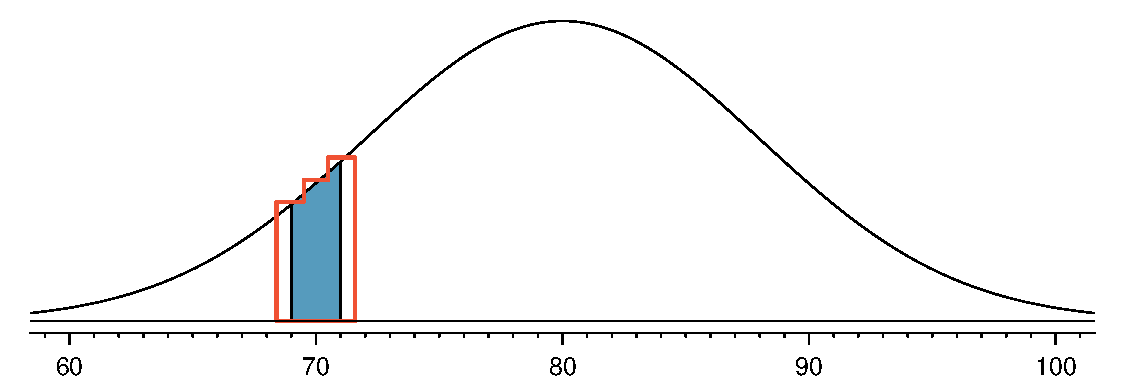
\includegraphics[width=\textwidth]{ch_distributions/figures/normApproxToBinomFail/normApproxToBinomFail}
\caption{A normal curve with the area between 69 and 71 shaded. The outlined area represents the exact binomial probability.}
\label{normApproxToBinomFail}
\end{figure}


\index{distribution!binomial!normal approximation|)}
\index{distribution!binomial|)}



%_________________
\section{More discrete distributions}
\label{discreteModels}

\subsection{Negative binomial distribution}
\label{negativeBinomial}

\index{distribution!negative binomial|(}

The geometric distribution describes the probability of observing the first success on the $n^{th}$ trial. The \termsub{negative binomial distribution}{distribution!negative binomial} is more general: it describes the probability of observing the $k^{th}$ success on the $n^{th}$ trial.

\begin{termBox}{\tBoxTitle{Negative binomial distribution}
The negative binomial distribution describes the probability of observing the $k^{th}$ success on the $n^{th}$ trial:
\begin{eqnarray}
\P(\text{the $k^{th}$ success on the $n^{th}$ trial}) = {n-1 \choose k-1} p^{k}(1-p)^{n-k}
\label{negativeBinomialEquation}
\end{eqnarray}
where $p$ is the probability an individual trial is a success. All trials are assumed to be independent.}
\end{termBox}

%\textC{\pagebreak}

To check that if $X$ is negative binomial($k$, $p$), then
\[
	1 = \P(k\le X<\infty),
\]
we have to get into \emph{binomial series}, a topic often neglected in calculus courses, so we shall refrain.

The justification for the probability mass function of the negative binomial distribution is clear: if the $k$th success occurs on the $n$th trial then there is some choice of $k-1$ of the first $n-1$ trials to also be successes, and the remaining factors are as in the binomial distribution.

%\begin{tipBox}{\tipBoxTitle{Binomial versus negative binomial}
%In the binomial case, we typically have a fixed number of trials and instead consider the number of successes. In the negative binomial case, we examine how many trials it takes to observe a fixed number of successes and require that the last observation be a success.}
%\end{tipBox}

\subsection{Poisson distribution}
\label{poisson}

\index{distribution!Poisson|(}



\begin{termBox}{\tBoxTitle{Poisson distribution}
Suppose we are watching for events and the number of observed events follows a Poisson distribution with rate $\lambda$. Then
\begin{align*}
\P(\text{observe $k$ events}) = \frac{\lambda^{k} e^{-\lambda}}{k!}
\end{align*}
where $k$ may take a value 0, 1, 2, and so on, and $k!$ represents $k$-factorial, as described on page~\pageref{factorialDefinitionInTheBinomialSection}. The letter $e\approx2.718$ is the base of the natural logarithm. The mean and standard deviation of this distribution are $\lambda$ and $\sqrt{\lambda}$, respectively.}
\end{termBox}

The rigorous explanation of the Poisson distribution is as follows. If $\lambda=np$ where $n\to\infty$ and $p$ remains constant (so $p=\lambda/n\to 0$) then the binomial distribution with parameters $n$ and $p$ converges to Poisson in the following sense. For fixed $k$ (so $k$ is relatively small),
\[
	\binom{n}{k}p^k(1-p)^{n-k} \to e^{-\lambda}\frac{\lambda^k}{k!}
\]
\[
	e^{-\lambda} = \lim \left(1-\frac\lambda{n}\right)^n = (1-p)^n
\]
\[
	(1-p)^{-k} \approx 1^{-k} = 1
\]
So it remains to show
\[
	\frac{n!}{(n-k)!} p^k \sim \lambda^k = (np)^k
\]
where $a\sim b$ means $\lim_{n\to\infty} \frac{a}b=1$.
This simplifies to
\[
	\frac{n!}{(n-k)!} = n(n-1)(n-2)\dots (n-(k+1)) \sim n^k
\]
which is clearly true as $n\to\infty$ and $k$ stays fixed.
%\textC{\pagebreak}

The important fact that
\[
	1 = \P(0\le X<\infty)
\]
follows from the Taylor series
\[
	e^\lambda = \sum_{k=0}^\infty \frac{\lambda^k}{k!}.
\]

The expectation of $X$ that is Poisson($\lambda$) is $\lambda$, just like the binomial($n$, $p$) has expectation $np$.
We verify as follows, using $t=k-1$:
\begin{eqnarray*}
\E(X) &=& \sum_{k=0}^\infty k \frac{\lambda^{k} e^{-\lambda}}{k!} = \sum_{k=1}^\infty k \frac{\lambda^{k} e^{-\lambda}}{k!} =\sum_{t=0}^\infty (t+1) \frac{\lambda^{t+1} e^{-\lambda}}{(t+1)!}
\\
&=&\sum_{t=0}^\infty \frac{\lambda^{t+1} e^{-\lambda}}{t!} =\lambda \sum_{t=0}^\infty \frac{\lambda^{t} e^{-\lambda}}{t!} = 1.
\end{eqnarray*}
To find the standard deviation we need
\begin{eqnarray*}
	\E(X^2) &=& \sum_{k=0}^\infty k^2 \frac{\lambda^{k} e^{-\lambda}}{k!} = \sum_{k=1}^\infty k^2 \frac{\lambda^{k} e^{-\lambda}}{k!} = \sum_{t=0}^\infty (t+1)^2 \frac{\lambda^{t+1} e^{-\lambda}}{(t+1)!}
\\
&=& \sum_{t=0}^\infty (t+1) \frac{\lambda^{t+1} e^{-\lambda}}{t!} = \lambda (\E(X) + 1) = \lambda(\lambda+1)
\end{eqnarray*}
hence $\sigma^2 = \E(X^2)-(\E(X))^2 = \lambda(\lambda+1) - \lambda^2 = \lambda$. Thus, Poisson has the unusual property that its variance equals its mean.

%\begin{tipBox}{\tipBoxTitle{Is it Poisson?}
%A random variable may follow a Poisson distribution if we are looking for the number of events, the population that generates such events is large, and the events occur independently of each other.}
%\end{tipBox}

\index{distribution!Poisson|)}

\section[Applications]{Applications \sectionvideohref{youtube-ncktqQoPUeA&feature=youtu.be&t=517&list=PLkIselvEzpM5Gn-sHTw1NF0e8IvMxwHDW}}
The Poisson distribution is a popular model for risky events studied by actuaries, in the case where we know how many events happen on average but we do not have values of $n$ and $p$ to set up a binomial or normal distribution. Click on the camera icon above for a video showcasing Guided Practice \ref{doris_kung} and featuring an author of the present text.
\begin{exercise}{Car accidents.}\label{doris_kung}
Suppose car accidents happen on average 1 every 10,000 miles.
What is the probability that after driving 10,000 miles we have no car accidents?\footnote{We have $\lambda=1$ and $\P(X=0)=e^{-\lambda}\lambda^0/0! = 1/e$.}
\end{exercise}

\begin{example}{Sunny Day cards.}
The following example may come up in playing with Kindergarteners. Suppose there are five cards, two of which shows hair clips, and one each show scissors, hair brush, and comb.
Suppose you pick two cards at random. What is the probability that exactly one of them shows hair clips?
This is known as the hypergeometric distribution: the probability that $k= 1$, where $K=2$, $N=5$, and $n=2$, is
\[
	\frac{
		\binom{K}{k}
		\binom{N-K}{n-k}
	}{
		\binom{N}{n}
	}
	= 
	\frac{
		\binom{2}{1}
		\binom{5-2}{2-1}
	}{
		\binom{5}{2}
	}
	= 60\%.
\]
The probability of two hair clips is 10\% and thus the probability of no hair clips is 30\%.
In general the probability, when picking $n$ items from $N$ items without replacement, of picking $k$ of the $K$ many with a particular property $Q$, is
\[
	\frac{
		\binom{K}{k}
		\binom{N-K}{n-k}
	}{
		\binom{N}{n}
	}
\]
because there are $\binom{N}{n}$ total sets of $n$ that you can choose, all equally likely; and those sets in which you choose $k$ many with the property $Q$ are determined by which ones you chose with
property $Q$ ($\binom{K}{k}$ many sets of $k$) and which ones you chose without property $Q$ ($\binom{N-K}{n-k}$ many choices).
\end{example}

\begin{example}{Banking.}
	A bank portfolio contains a loan that has gone into default.
	Each time period a proportion $p_i$ of the outstanding balances are paid.
	Interest is not added to the outstanding balances (as that would be cruel, perhaps), but the bank loses money as the borrowers take a long time to repay.
	The proportion of funds recovered by the bank is, in terms of a discount rate $d=1/(1+r)$ (where $r>0$ is an interest rate),
	\[
		s = p_0 + (1-p_0)p_1d + (1-p_0)(1-p_1)p_2d^2+\dots = \sum_{i=0}^\infty d^i p_i\prod_{j=0}^{i-1} (1-p_j)
	\]
	Suppose $p_i$ are independent random variables. Then
	\begin{eqnarray*}
		\E(s)&=&\sum_{i=0}^\infty d^i \E\left(p_i\prod_{j=0}^{i-1} (1-p_j)\right)\\
		&=& \sum_{i=0}^\infty d^i \E(p_i)\prod_{j=0}^{i-1} (1-\E(p_j)).
	\end{eqnarray*}
	Calculate $\E(s)$ when each $\E(p_i)=1/2$ and $r=1/2$.\footnote{We have $\prod_{j=0}^{i-1}(1-\E(p_j))=2^{-i}$ and $d=2/3$, so
	\[
		\E(s)=\sum_{i=0}^\infty (2/3)^i (1/2)(1/2)^i = (1/2)\sum_{i=0}^\infty (1/3)^i = (1/2)\frac1{1-\frac13} = \frac34.
	\]
	}
\end{example}

\begin{example}{Earned premium.}\label{drc}
	An insurance company offers flood insurance at a cost (premium) of $c=\$100$.
	The insurance is good for one year. Each month there is a probability $p$ of a flood leading to a $\$100,000$ payout.
	As the months go by, the insurance company considers that it is earning the premium in a linear fashion:
	after $k$ months, $c\frac{k}{12}$ has been earned.
	Assume that no more than one payout can be made in a year on the same policy.
	Find the probability distribution of the amounth earned after 6 months.
	For which value of $p$ is the expected amount earned after 6 months equal to 0?\footnote{
		$\$50$ will have been earned if there is no flood.
		If there has been a flood, then $\$100-\$100,000$ will have been earned.
		Thus, if $X$ is the amount earned then
		$P(X=k)=(1-p)^6\cdot 1_{k=\$50} + (1-(1-p)^6)\cdot 1_{k=-\$99,900}$.
		The expectation is $0=E(X)=\$50 (1-p)^6 - \$99,900\cdot (1-(1-p)^6)$.
		This gives, for $\alpha=(1-p)^6$, that $0=50\alpha-99900(1-\alpha)$ and hence
		$99900=99950\alpha$, $\alpha=\frac{99900}{99950}=\frac{9990}{9995}=\frac{1998}{1999}$.
		Hence $p=1-\left(\frac{1998}{1999}\right)^{1/6}\approx 0.000083$.
	}
\end{example}
\begin{example}{Earned premium, two policies.}
	Suppose Kaden purchases the flood insurance in Example \ref{drc}. Kaden's friend Tamzin decides to purchase the same insurance
	but have it be effective 6 months after Kaden's insurance becomes effective. She is in effect betting that there will be no
	flood during the first 6 months.
	What is the expected earned premium for the insurance company 9 months after Kaden purchased his insurance?
	Is it 0 for the same $p$ as in the above example?
	Assume that Kaden and Tamzin are neighbors, so that any flood affects them equally.
	%\footnote{
	Solution:
		Let $X$ be now the amount earned after 9 months.
		Let $F_1$ be the event of a flood in the first 6 months, and $F_2$ be the event of a flood in the subsequent 3 months.
		There are three cases:
		$F_1\cap F_2$,
		$F_1\setminus F_2$,
		$F_2\setminus F_1$,
		$\bar{F_1}\cap\bar{F_2}$.
		These have probability
		$(1-(1-p)^6)(1-(1-p)^3)$,
		$(1-(1-p)^6)(1-p)^3$,
		$(1-p)^6(1-(1-p)^3)$, and
		$(1-p)^6(1-p)^3=(1-p)^9$, respectively.
		The respective earned premiums are
		$2(100-100,000)$,
		$100+25-100,000$,
		$2(100-100,000)$,
		$75+25$.
		
		The expected earned premium $E(X)$ is then, in terms of $\beta=(1-p)^3$, and $f=100-100,000$,
		\[
		2(100-100,000) (1-\beta^2)(1-\beta) +
		(100+25-100,000) (1-\beta^2)\beta
		\]
		\[ +
		2(100-100,000) \beta^2(1-\beta) +
		(75+25)(\beta^3)
		\]
		\[
			= 2f(1-\beta) + (25+f)(1-\beta^2)\beta + 100\beta^3.
		\]
		\[
			= 2f + (25-f)\beta + (100-25-f)\beta^3
		\]
		which according to WolframAlpha (input:
			\verb!(75+99900)x**3+(25+99900)x+2(-99900)!)
		is 0 when $\beta\approx 0.99975$. In other words,
		$p\approx 1-(0.99975)^{1/3}=0.0000833403$.
	%}
	\begin{example}{CEO effort.}
		This example is taken from the paper \emph{The Contract Disclosure Mandate and Earnings Management under External Scrutiny}
		by Tae Wook Ryan Kim and Carlos Corona, \verb!http://hdl.handle.net/10125/64934!.
		\begin{quote}
		We consider a single-period contracting setting with three kinds of players:
		$N$ identical principals (or shareholders, referred to as ``she''),
		$N$ identical agents (or managers, referred to as ``he''), and one inspector.
		All agents are risk- averse and all other parties are risk-neutral.
		In any firm $i \in \{1,\dots,N\}$, the principal needs to hire an agent to operate it.
		All principals simultaneously, each one to a different agent, make a take-it-or-leave-it contract offer.
		Each agent can either accept or reject the offer. If the agent rejects the offer, the game ends.
		If the agent accepts the contract offer, he chooses a level of effort, $a_i$, which is only observed by the agent himself.
		Productive effort affects true earnings $e_i = va_i + \epsilon_i$ , where $\epsilon_i\sim N(0,\sigma^2)$\footnote{A normal random variable with variance $\sigma^2$ and mean 0} is a random component of earnings that the agent cannot control, and $v > 0$ is the true earnings sensitivity to effort.
		\end{quote}
		If we take $\sigma=1$ and $v=1$, what effort $a_i$ is needed to ensure that with 95\% probability, the earnings are greater than 1?\footnote{We need $95\%=P(e_i>1)=P(a_i+\epsilon_i>1)=P(\epsilon_i>1-a_i)=1-\Phi(1-a_i)$. Thus $\Phi(1-a_i)=1/20$ and $a_i=1-\Phi^{-1}(1/20)$.
		We cannot directly apply the 68-95-99.7 rule, as we would need a 90 rule.
		From a table or from the command \texttt{=norminv(0.05,0,1)} we see that $\Phi^{-1}(1/20)=-1.645$.
		Thus $a_i=2.645$.
		}
	\end{example}
\end{example}